\documentclass[10pt]{article}
% header.tex
% this is where you load pacakges, specify custom formats, etc.

\usepackage[left=1in,right=1in,top=1in,footskip=25pt]{geometry} 
% \usepackage{changepage}
\usepackage{amsmath,amsthm,amssymb,amsfonts}
\usepackage{mathtools}
\usepackage{bm}
\usepackage{bbm}
\usepackage{mathrsfs}
\usepackage{accents}
\usepackage{xspace}
% enumitem for custom lists
\usepackage{enumitem}
% Load dsfont this to get proper indicator function (bold 1) with \mathds{1}:
\usepackage{dsfont}
\usepackage{centernot}

\usepackage[ruled,vlined,linesnumbered]{algorithm2e}
\usepackage{multirow}
\usepackage{booktabs}
\makeatletter
% Booktab style
\renewcommand*{\@algocf@pre@ruled}{\hrule height\heavyrulewidth depth0pt \kern\belowrulesep}
\renewcommand*{\algocf@caption@ruled}{\box\algocf@capbox\kern\aboverulesep\hrule height\lightrulewidth\kern\belowrulesep}
\renewcommand*{\@algocf@post@ruled}{\kern\aboverulesep\hrule height\heavyrulewidth\relax}
\makeatother

\usepackage[usenames,dvipsnames]{xcolor}

% set up commenting code (I will use this during marking)
\definecolor{CommentColor}{rgb}{0,.50,.50}
\newcounter{margincounter}
\newcommand{\displaycounter}{{\arabic{margincounter}}}
\newcommand{\incdisplaycounter}{{\stepcounter{margincounter}\arabic{margincounter}}}
\newcommand{\COMMENT}[1]{\textcolor{CommentColor}{$\,^{(\incdisplaycounter)}$}\marginpar{\scriptsize\textcolor{CommentColor}{ {\tiny $(\displaycounter)$} #1}}}

\usepackage{appendix}

% set up graphics
\usepackage{graphicx}
\DeclareGraphicsExtensions{.pdf,.png,.jpg}
\graphicspath{{fig/}}
\usepackage{float}

\usepackage[sorting=ynt,backend=biber,bibstyle=apa,citestyle=apa,giveninits=true,sortcites]{biblatex}
\setlength\bibitemsep{1.5\itemsep}

\usepackage{fancyhdr}
\pagestyle{fancy}
%\fancyhead[L]{}
\setlength{\headheight}{40pt}

%%%%%%%%%%%%%%%%%%%%%%%%%%%%%%%%%%%%%%%%%%%%%%%%%%%%%%%%%%%%%%%%%%%%%%%%%%%%%%%%%%%%
% most other packages you might use should be loaded before hyperref
%%%%%%%%%%%%%%%%%%%%%%%%%%%%%%%%%%%%%%%%%%%%%%%%%%%%%%%%%%%%%%%%%%%%%%%%%%%%%%%%%%%%

% Set up hyperlinks:
\definecolor{RefColor}{rgb}{0,0,.65}
\usepackage[colorlinks,linkcolor=RefColor,citecolor=RefColor,urlcolor=RefColor]{hyperref}

\usepackage[capitalize]{cleveref}
\crefname{appsec}{Appendix}{Appendices} % you can tell cleveref what to call things

\renewenvironment{abstract}
 {\par\noindent\textbf{\abstractname.}\ \ignorespaces}
 {\par\medskip}
 
 \setlength\parindent{0pt}
% defs.tex
% this is where you define custom notation, commands, etc.


%%
% full alphabets of different styles
%%

% bf series
\def\bfA{\mathbf{A}}
\def\bfB{\mathbf{B}}
\def\bfC{\mathbf{C}}
\def\bfD{\mathbf{D}}
\def\bfE{\mathbf{E}}
\def\bfF{\mathbf{F}}
\def\bfG{\mathbf{G}}
\def\bfH{\mathbf{H}}
\def\bfI{\mathbf{I}}
\def\bfJ{\mathbf{J}}
\def\bfK{\mathbf{K}}
\def\bfL{\mathbf{L}}
\def\bfM{\mathbf{M}}
\def\bfN{\mathbf{N}}
\def\bfO{\mathbf{O}}
\def\bfP{\mathbf{P}}
\def\bfQ{\mathbf{Q}}
\def\bfR{\mathbf{R}}
\def\bfS{\mathbf{S}}
\def\bfT{\mathbf{T}}
\def\bfU{\mathbf{U}}
\def\bfV{\mathbf{V}}
\def\bfW{\mathbf{W}}
\def\bfX{\mathbf{X}}
\def\bfY{\mathbf{Y}}
\def\bfZ{\mathbf{Z}}

\def\bfb{\mathbf{b}}
\def\bfe{\mathbf{e}}
\def\bfg{\mathbf{g}}
\def\bft{\mathbf{t}}
\def\bfx{\mathbf{x}}
\def\bfy{\mathbf{y}}
\def\bfz{\mathbf{z}}

\def\bfom{\bm{\omega}}
\def\bfOm{\bm{\Omega}}

% bb series
\def\bbA{\mathbb{A}}
\def\bbB{\mathbb{B}}
\def\bbC{\mathbb{C}}
\def\bbD{\mathbb{D}}
\def\bbE{\mathbb{E}}
\def\bbF{\mathbb{F}}
\def\bbG{\mathbb{G}}
\def\bbH{\mathbb{H}}
\def\bbI{\mathbb{I}}
\def\bbJ{\mathbb{J}}
\def\bbK{\mathbb{K}}
\def\bbL{\mathbb{L}}
\def\bbM{\mathbb{M}}
\def\bbN{\mathbb{N}}
\def\bbO{\mathbb{O}}
\def\bbP{\mathbb{P}}
\def\bbQ{\mathbb{Q}}
\def\bbR{\mathbb{R}}
\def\bbS{\mathbb{S}}
\def\bbT{\mathbb{T}}
\def\bbU{\mathbb{U}}
\def\bbV{\mathbb{V}}
\def\bbW{\mathbb{W}}
\def\bbX{\mathbb{X}}
\def\bbY{\mathbb{Y}}
\def\bbZ{\mathbb{Z}}

% cal series
\def\calA{\mathcal{A}}
\def\calB{\mathcal{B}}
\def\calC{\mathcal{C}}
\def\calD{\mathcal{D}}
\def\calE{\mathcal{E}}
\def\calF{\mathcal{F}}
\def\calG{\mathcal{G}}
\def\calH{\mathcal{H}}
\def\calI{\mathcal{I}}
\def\calJ{\mathcal{J}}
\def\calK{\mathcal{K}}
\def\calL{\mathcal{L}}
\def\calM{\mathcal{M}}
\def\calN{\mathcal{N}}
\def\calO{\mathcal{O}}
\def\calP{\mathcal{P}}
\def\calQ{\mathcal{Q}}
\def\calR{\mathcal{R}}
\def\calS{\mathcal{S}}
\def\calT{\mathcal{T}}
\def\calU{\mathcal{U}}
\def\calV{\mathcal{V}}
\def\calW{\mathcal{W}}
\def\calX{\mathcal{X}}
\def\calY{\mathcal{Y}}
\def\calZ{\mathcal{Z}}

\def\tildeU{\widetilde{U}}
\def\hatb{\widehat{\bfb}}
\def\hatOm{\widehat{\bfOm}}
\def\hatW{\widehat{\bfW}}
\def\hatmu{\widehat{\mu}}


%%%%%%%%%%%%%%%%%%%%%%%%%%%%%%%%%%%%%%%%%%%%%%%%%%%%%%%%%%
% text short-cuts
\def\iid{i.i.d.\ } %i.i.d.
\def\ie{i.e.\ }
\def\eg{e.g.\ }
\def\Polya{P\'{o}lya\ }
%%%%%%%%%%%%%%%%%%%%%%%%%%%%%%%%%%%%%%%%%%%%%%%%%%%%%%%%%%

%%%%%%%%%%%%%%%%%%%%%%%%%%%%%%%%%%%%%%%%%%%%%%%%%%%%%%%%%%
% quasi-universal probabilistic and mathematical notation
% my preferences (modulo publication conventions, and clashes like random vectors):
%   vectors: bold, lowercase
%   matrices: bold, uppercase
%   operators: blackboard (e.g., \mathbb{E}), uppercase
%   sets, spaces: calligraphic, uppercase
%   random variables: normal font, uppercase
%   deterministic quantities: normal font, lowercase
%%%%%%%%%%%%%%%%%%%%%%%%%%%%%%%%%%%%%%%%%%%%%%%%%%%%%%%%%%

% operators
\def\P{\bbP} %fundamental probability
\def\E{\bbE} %expectation
% conditional expectation
\DeclarePairedDelimiterX\bigCond[2]{[}{]}{#1 \;\delimsize\vert\; #2}
\newcommand{\conditional}[3][]{\bbE_{#1}\bigCond*{#2}{#3}}
\def\Law{\mathcal{L}} %law; this is by convention in the literature
\def\indicator{\mathds{1}} % indicator function

% sets and groups
\def\borel{\calB} %Borel sets
\def\sigAlg{\calA} %sigma-algebra
\def\filtration{\calF} %filtration
\def\grp{\calG} %group

% binary relations
\def\condind{{\perp\!\!\!\perp}} %independence/conditional independence
\def\equdist{\stackrel{\text{\rm\tiny d}}{=}} %equal in distribution
\def\equas{\stackrel{\text{\rm\tiny a.s.}}{=}} %euqal amost surely
\def\simiid{\sim_{\mbox{\tiny iid}}} %sampled i.i.d

% common vectors and matrices
\def\onevec{\mathbf{1}}
\def\iden{\mathbf{I}} % identity matrix
\def\supp{\text{\rm supp}}

% misc
% floor and ceiling
\DeclarePairedDelimiter{\ceilpair}{\lceil}{\rceil}
\DeclarePairedDelimiter{\floor}{\lfloor}{\rfloor}
\newcommand{\argdot}{{\,\vcenter{\hbox{\tiny$\bullet$}}\,}} %generic argument dot

\DeclareMathOperator*{\argmax}{arg\,max}
\DeclareMathOperator*{\argmin}{arg\,min}
%%%%%%%%%%%%%%%%%%%%%%%%%%%%%%%%%%%%%%%%%%%%%%%%%%%%%%%%%%

%%%%%%%%%%%%%%%%%%%%%%%%%%%%%%%%%%%%%%%%%%%%%%%%%%%%%%%%%%
%% some distributions
% continuous
\def\UnifDist{\text{\rm Unif}}
\def\BetaDist{\text{\rm Beta}}
\def\ExpDist{\text{\rm Exp}}
\def\GammaDist{\text{\rm Gamma}}
% \def\GenGammaDist{\text{\rm GGa}} %Generalized Gamma

% discrete
\def\BernDist{\text{\rm Bernoulli}}
\def\BinomDist{\text{\rm Binomial}}
\def\PoissonPlus{\text{\rm Poisson}_{+}}
\def\PoissonDist{\text{\rm Poisson}}
\def\NBPlus{\text{\rm NB}_{+}}
\def\NBDist{\text{\rm NB}}
\def\GeomDist{\text{\rm Geom}}
% \def\CRP{\text{\rm CRP}}
% \def\EGP{\text{\rm EGP}}
% \def\MittagLeffler{\text{\rm ML}}
%%%%%%%%%%%%%%%%%%%%%%%%%%%%%%%%%%%%%%%%%%%%%%%%%%%%%%%%%%

%%%%%%%%%%%%%%%%%%%%%%%%%%%%%%%%%%%%%%%%%%%%%%%%%%%%%%%%%%
% Project-specific notation should go here
% (Because it's at the end of the file, it can overwrite anything that came before.)

%e.g.,
\def\Laplacian{\calL}
%\def\P{\calP}

% combinatorial objects
\def\perm{\sigma} %fixed permutation
\def\Perm{\Sigma} %random permutation
\def\part{\pi} %fixed partition
\def\Part{\Pi} %random partition

% Kernels
\def\MMD{\mathrm{MMD}}
\def\hatMMD{\widehat{\MMD}}
\def\dhatMMD{\widehat{\vphantom{\rule{1.5pt}{5.5pt}}\smash{\hatMMD}}}
\def\d{\mathrm{d}}

\def\xo{x^{(1)}}
\def\xt{x^{(2)}}
\def\yo{y^{(1)}}
\def\yt{y^{(2)}}
\def\go{g^{(1)}}
\def\gtw{g^{(2)}}

% Theorems
\newtheorem{theorem}{Theorem}[section]
\newtheorem{proposition}[theorem]{Proposition}
\newtheorem{corollary}[theorem]{Corollary}
\renewcommand{\thetheorem}{\arabic{theorem}}


\newcommand{\mre}{\textsc{MRE}\xspace}
\newcommand{\Var}{\mathrm{Var}}
\newcommand{\bias}{\mathrm{bias}}
\newcommand{\barY}{\bar{Y}}

\newcommand{\T}{\top}

\newcommand\sbullet[1][.5]{\mathbin{\vcenter{\hbox{\scalebox{.75}{$\bullet$}}}}}

% Network interference
\newcommand{\Ni}{\calN_i}
\newcommand{\Nmi}{\calN_{-i}}
\newcommand{\ZNi}{\bfZ_{\calN_i}}
\newcommand{\ZNmi}{\bfZ_{\calN_{-i}}}
\newcommand{\YNi}{\bfY_{\calN_i}}
\newcommand{\YNmi}{\bfY_{\calN_{-i}}}
\newcommand{\Xind}{\bfX^{\text{ind}}}
\newcommand{\Xneigh}{\bfX^{\text{neigh}}}
\newcommand{\Yobs}{\bar{Y}^{\text{obs}}_{z,g}}

\newcommand{\tausutva}{\tau_\text{sutva}}

%%%%%%%%%%%%%%%%%%%%%%%%%%%%%%%%%%%%%%%%%%%%%%%%%%%%%%%%%%

\newcommand{\todo}{{\color{red}{TODO}}}

\usepackage{tikz}

\title{Estimating treatment effects from observational network data\\\vspace{0.5em}\large{STAT 548 Qualifying Paper}}
\author{Kenny Chiu}
\date{\today}

\bibliography{refs.bib}

\begin{document}

\maketitle

\vspace{2em}

\begin{abstract}
\textcite{Forastiere:2021} examine the problem of estimating causal treatment effects from observational network data in the presence of interference. We review their proposed method and discuss its place in the literature. We present simple examples that illustrate the relevance of their theoretical results. We replicate part of their simulation study on a different dataset (the Twitch social network dataset), obtain findings mostly consistent with theirs, and discuss the possible reasons for the few inconsistent results. We also provide a critique of their work.
\end{abstract}

\vspace{2em}


\section{Introduction}

\textcite{Forastiere:2021} examine the problem of estimating causal treatment effects from observational network data in the presence of interference. The problem is formulated under a potential outcome framework in which they propose a propensity score-based estimator for the treatment effect that is unbiased under certain assumptions. \citeauthor{Forastiere:2021} also derive the biases of naive estimators that ignore interference under their framework. In this report, we review the work by \textcite{Forastiere:2021}, present simple examples that illustrate their theoretical results, and replicate part of their simulation study on a different dataset.
\\

This report is organized as follows: Section~\ref{sec:notation} introduces the notation used in this report; Section~\ref{sec:summary} summarizes their proposed methodology in the context of the literature; Section~\ref{sec:example} presents examples that illustrate the relevance of their theoretical results; Sections~\ref{sec:simulation} and \ref{sec:extension} discusses our attempts at replicating part of their simulation study on a different dataset; and Section~\ref{sec:critique} concludes the report with a critique of their work. Appendix~\ref{apx:example} includes our technical derivations from Section~\ref{sec:example}, and Appendix~\ref{apx:simulation} contains additional information about the dataset and our simulations from Sections~\ref{sec:simulation} and \ref{sec:extension}.


\section{Notation} \label{sec:notation}

Throughout this report, we closely follow the notation used by \textcite{Forastiere:2021}. Let $G=(\calN,\calE)$ be an undirected network where $\calN$ is a set of $N$ units (nodes) and $\calE=\{\{i,j\}: i,j\in\calN\}$ is a set of edges. For a unit $i\in\calN$, a partition~$(i,\Ni,\Nmi)$ of $\calN$ describes unit~$i$'s neighbourhood~$\calN_i$ (the set of $N_i$ units connected to unit $i$) and the set~$\calN_{-i}$ of all other units that are not $i$ and that are not in $\calN_i$. Let $Z_i\in\{0,1\}$ be the treatment assigned to unit $i$ and $Y_i\in\calY$ the observed outcome of unit $i$.
Denote the treatment vector for the population~$\calN$ as $\bfZ$ and the corresponding vectors for partition~$(i,\Ni,\Nmi)$ as $(Z_i,\ZNi,\ZNmi)$.
%Denote the treatment and outcome vector for the population~$\calN$ as $\bfZ$ and $\bfY$, respectively, and the corresponding vectors for partition~$(i,\Ni,\Nmi)$ as $(Z_i,\ZNi,\ZNmi)$ and $(Y_i,\YNi,\YNmi)$.
Let $G_i=g_i(\ZNi)\in\calG_i$ be some known and well-specified summary~$g_i$ of the treatments in unit~$i$'s neighbourhood.
%, and denote the vector of neighbourhood treatments for the population as $\bfG$
Depending on the size of a unit's neighbourhood, the space $\calG_i$ may differ between units. Let $V_g=\{i\in\calN:g\in\calG_i\}$ denote the subset containing $v_g$ units that have $g$ as a possible value for the neighbourhood treatment. Let $\bfX_i\in\calX$ be a vector of covariates for unit~$i$ that partitions into individual-level characteristics $\Xind_i\in\calX^\text{ind}$ and neighbourhood-level/aggregated individual-level characteristics $\Xneigh_i\in\calX^\text{neigh}$.
\\

We use $\E[\argdot]$ and $\P(\argdot)$ to denote expectations and probabilities, respectively. Note that in the context of a given network, these quantities should be viewed from the ``super-population'' perspective \parencite{Imbens:2015} and are defined in terms of averages over the finite network. Otherwise, expectations and probabilities are interpreted the conventional way. We leave it up to the context to distinguish which interpretation is used throughout this report.


\section{Review of proposed methodology} \label{sec:summary}

In this section, we explain the method proposed by \textcite{Forastiere:2021} and discuss its relevance in the context of the related literature. We also discuss its advantages over other methods used in similar contexts.

\subsection{Setting, objective and method}\label{sec:method}

\textcite{Forastiere:2021} focus on the problem of estimating treatment effects from observational network data under interference. The setting is challenging for causal inference because
\begin{enumerate}
\item
the assignment mechanism of treatments is unknown with observational data and so estimated effects may be biased in the presence of unmeasured confounders, and
\item
conventional inference methods typically ignore the effect of interference, which may also lead to biased estimates.
\end{enumerate}
In the randomized controlled trial literature, these issues can generally be dealt with by designing the study in such a way that the influence of confounders is minimized and that inference methods that do account for interference can be used \parencite[e.g.,][]{Saveski:2017,Jagadeesan:2020,Imai:2021,Doudchenko:2020}. In the observational setting, these considerations need to be addressed by the inference method in the analysis phase. \citeauthor{Forastiere:2021} specifically focus on the setting involving a binary treatment (e.g., an intervention and a control) and where the interference on a unit comes from only its treated neighbours. They formulate the inference problem under a potential outcome framework, and they propose an estimation procedure that yields unbiased treatment and spillover (interference) effect estimates under certain assumptions.
\\

%Their procedure for estimating effects is based on matching units into sets based on covariate values, compute the effect contrast within each matched set, and estimate the effect by the (weighted) average of the contrasts across sets. However, matching may be difficult when the space of possible covariate values is large or if there are many covariates.
The procedure proposed by \textcite{Forastiere:2021} involves partitioning units into subclasses according to a joint propensity score~$\psi(z;g;x)$ that they also define. The joint propensity score factorizes into a neighbourhood propensity score~$\lambda(g;z;\bfx^g)$ (probability of being exposed to neighbourhood treatment $g$ given individual treatment $z$ and relevant covariates $\bfx^g$) and an individual propensity score~$\phi(z;\bfx^z)$ (probability of being assigned treatment $z$ given relevant covariates $\bfx^z$), which they exploit in order to avoid adjusting for all covariates at once and needing to work in a higher-dimensional space. Note that $\bfX^g$ and $\bfX^z$ do not necessarily correspond to $\Xneigh$ and $\Xind$, respectively, as they may not be disjoint. The steps for their propensity score-based estimation procedure are as follows:
\begin{enumerate}

\item
\textbf{Subclassify units}.
\begin{enumerate}
\item
Fit a logistic regression model on the individual treatments~$Z_i$ given covariates~$\bfX_i^z$, and use the model to predict the individual propensity scores~$\phi(1;\bfX_i^z)$.
\item
Partition the units into $J$ subclasses $B_j$, $j\in\{1,\ldots,J\}$, based on similar estimated individual propensity scores~$\hat{\phi}(1;\bfX_i^z)$ and such that each subclass is approximately balanced in the number of treated and untreated units.
\end{enumerate}

\item
\textbf{Estimate potential outcomes}. Let $B_j^g=	V_g\cap B_j$. For each subclass~$B_j$:
\begin{enumerate}
\item
Fit some regression model on the neighbourhood treatments $G_i$ given the individual treatments~$Z_i$ and covariates~$\bfX_i^g$, and use the model to estimate the neighbourhood propensity scores~$\lambda(g;z;\bfX_i^g)$.
\item
Fit some regression model on the potential outcomes~$Y_i(z,g)$ given the individual and neighbourhood treatments~$Z_i$ and $G_i$ and the estimated neighbourhood propensity scores~$\hat{\lambda}(g;z;\bfX_i^g)$.
\item
Estimate the dose-response function by averaging over the estimated potential outcomes for a particular level of the joint treatment, i.e.,
\[
\hat{\mu}_j(z,g;V_g) = \frac{\sum_{i\in B_j^g}\hat{Y}_i(z,g)}{\left|B_j^g\right|}\;.
\]
\end{enumerate}

\item
\textbf{Estimate the average dose-response function} (ADRF) $\mu(z,g;V_g)=\E\left[Y_i(z,g)|i\in V_g\right]$ for a particular level of the joint treatment by taking the weighted average of the estimated dose-response functions over the subclasses, i.e.,
\[
\hat{\mu}(z,g;V_g) = \sum_{j=1}^J\hat{\mu}_j(z,g;V_g)\left(\frac{\left|B_j^g\right|}{v_g}\right) \;.
\]

\item
\textbf{Estimate} the treatment effects $\tau(g)$, overall treatment effect $\tau$, spillover effects $\delta(g;z)$ and overall spillover effects $\Delta(z)$ using the estimated ADRF by
\begin{align*}
\hat{\tau}(g) &= \hat{\mu}(1,g;V_g) - \hat{\mu}(0,g;V_g) \;, & \hat{\tau}&=\sum_{g\in\calG}\hat{\tau}(g)\P(G_i=g) \;, \\
\hat{\delta}(g;z) &= \hat{\mu}(z,g;V_g) - \hat{\mu}(z,0;V_g) \;, & \hat{\Delta}(z) &= \sum_{g\in\calG}\hat{\delta}(g;z)\P(G_i=g)\;.
\end{align*}

\end{enumerate}
\textcite{Forastiere:2021} show that their estimators for the treatment and spillover effects are unbiased under three assumptions, the first two of which form the Stable Unit Treatment on Neighbourhood Value Assumption (SUTNVA, a generalization of SUTVA that relaxes the no interference assumption to allow interference of immediate neighbours) and the third being an unconfoundedness assumption that says the treatment assignment mechanism is conditionally independent of the outcomes for the given set of covariates.

\subsection{In context of the literature}

The body of literature that involves estimating causal treatment effects from observational data under general forms of interference is still relatively new. We summarize the common approaches in this literature and discuss how the work by \textcite{Forastiere:2021} fits in. We also briefly highlight other work that examine similar problems under different but closely related contexts.

\subsubsection{Similar contexts}

As noted by \textcite{Forastiere:2021}, the majority of works that look at similar problems under the same context involve either inverse probability-weighted (IPW) estimators \parencite{Liu:2016} or targeted maximum likelihood estimators (TMLE) \parencite{VanDerLaan:2014,Sofrygin:2017,Ogburn:2017} for the causal treatment effect. The main advantage of the method proposed by \citeauthor{Forastiere:2021} over these two approaches is the weaker assumptions that it requires.
\\

IPW estimators are weighted averages of the outcomes where the weights are defined with respect to a hypothetical allocation strategy (an assumed distribution over the neighbourhood treatments) and a known or correctly modelled generalized propensity score. The Bernoulli allocation strategy \parencite{Tchetgen:2012} is commonly used, which assumes that each unit in the neighbourhood is treated independently with probability $\alpha$ and that a unit's assignment is independent of its neighbours' assignment. This assumption rules out homophily---the tendency for units with similar characteristics to form ties---which is a strong assumption that is said to be unrealistic \parencite{Shalizi:2011}. In contrast, the estimators proposed by \textcite{Forastiere:2021} only use the observed neighbourhood treatments, and therefore no assumptions that explicitly rule out homophily are made (though the issue may still manifest as an unmeasured confounder if the unconfoundedness assumption does not hold for the given set of covariates). Both the IPW estimators and the estimators proposed by \citeauthor{Forastiere:2021} rely on being able to correctly model the joint propensity score.
\\

TMLEs are obtained by maximizing the likelihood of the outcomes defined on a structural equation model. Similar to the IPW estimators, TMLE generally involves a randomization assumption \parencite{VanDerLaan:2014} on the model where the conditional joint distribution of the treatment assignments factorizes into independent conditionals given the covariates for all units, and similarly for the conditional joint distribution of the outcomes given the covariates and the treatment assignments. In comparison, the unconfoundedness assumption in the method proposed by \textcite{Forastiere:2021} makes a weaker assumption where the outcome and treatment assignment of each unit is conditionally independent given only the covariates of that unit. The significance of these assumptions again circle back to the argument of disregarding homophily and/or other venues of confounding. It is notable that extensions of TMLE that allow for limited forms of homophily were later introduced \parencite{Ogburn:2017}.
\\

More recently, approaches that can be described as extensions of the method by \textcite{Forastiere:2021} have been proposed. \textcite{Jackson:2020} proposed estimators based on propensity score matching but which also explicitly account for homophily by modeling neighbourhood treatment assignments as an incomplete information game. \textcite{Sanchez:2021} questioned the justification of the unconfoundedness assumption with respect to the constructed propensity score (which would need to be estimated for every unit in the network and may be challenging to estimate accurately) and proposed a two-step method where a network propensity score is estimated and then used to as inverse weights to match units.

\subsubsection{Other contexts}

We briefly highlight other works in the literature that look at similar problems under different but closely related contexts. The difference in settings makes it difficult to directly compare these approaches to that proposed by \textcite{Forastiere:2021}.
\\

A large body of the literature examine the inference problem under the assumption of partial interference where units are partitioned into groups with no spillover effects between groups. The focus on partial interference settings seems to be primarily due to momentum of earlier works \parencite[e.g.,][]{Sobel:2006,Hudgens:2008} that looked at inference in randomized control studies with interference in which group-randomization tends to be more practical. Examples of recent work that assume partial interference include the work by \textcite{Liu:2019}, \textcite{Barkley:2020}, and \textcite{Qu:2021}. IPW estimators are commonly used in the partial interference setting as they were originally introduced for grouped observational data \parencite{Tchetgen:2012}.
\\

A small number of works consider more specific and niche contexts. For example, \textcite{Toulis:2018} explore the problem of treatment entanglement (where treatment assignments are assumed to satisfy certain restrictions) and proposes a propensity score-based estimator. \textcite{Zigler:2021} focus on the problem of bipartite causal inference with interference (where the treatment is applied to one unit and the outcome is measured on another) and propose a IPW estimator for this setting.
%Outside of the observational setting, there are many works that study causal inference in randomized studies with potential interference. These works generally examine study designs that allow for treatment effect estimation in the presence of interference under varying contexts \parencite[e.g.,][]{Saveski:2017,Jagadeesan:2020,Imai:2021,Doudchenko:2020}


\section{Potential bias of naive estimator}\label{sec:example}

In this section, we describe a simple example that illustrates the relevance of Theorem~2.A, Corollary~2 and Corollary~3 in the paper by \textcite{Forastiere:2021}. Specifically, we show for a simple network that
\begin{enumerate}

\item
if the unconfoundedness assumption holds but the individual and neighbourhood treatments are not conditionally independent for a given set of covariates, then an unbiased naive estimator that assumes SUTVA for the treatment effect will be biased due to interference effects, and

\item
if the individual and neighbourhood treatments are conditionally independent but the unconfoundedness assumption does not hold for a given set of covariates, then an unbiased SUTVA estimator will be biased due to unmeasured confounders.

\end{enumerate}

Consider some undirected network $G=(\calN,\calE)$ where every unit is paired (has an edge) with exactly one other unit. For simplicity, we index a unit by its pair $i\in\bbN$ and its position $j\in\{1,2\}$ within the pair. Denote $Z_{ij}\in\{0,1\}$ as the treatment assignment of unit $j$ in pair $i$. Let the neighbourhood treatment~$G_{ij}$ denote whether unit $(ij)$'s paired counterpart is treated. Therefore, $\calG_{ij}=\{0,1\}$ for all units in the network and $V_g=\calN$ for all $g\in\{0,1\}$. For convenience of notation, we drop the dependence on $V_g$ where applicable. Let $\bfX_{ij}=X_{ij}\in\{0,1\}$ be some measured covariate for each unit, and assume that the covariates of the units in the network are generated independently with $\P(X_{ij}=1)=\P(X_{ij}=0)=\frac{1}{2}$. Let $Y_{ij}\in\bbR$ be the outcome measured for each unit. Other details, such as the size of $\calN$, are assumed but left unspecified due to being irrelevant for the discussion. Figure~\ref{fig:example} shows an example network.
\\

\begin{figure}[ht]
\centering
\begin{tikzpicture}[thick,main/.style={draw,circle},node distance={6.5em},minimum size={1cm}]
\node[main,align=center,label={[yshift=-0.25em,align=center]$X_{11}=1$\\$Y_{11}=y_{11}$}] (11) {$Z_{11}=1$\\$G_{11}=0$};
\node[main,align=center,label={[yshift=-7.75em,align=center]$X_{12}=0$\\$Y_{12}=y_{12}$}] (12) [below of=11] {$Z_{12}=0$\\$G_{12}=1$};
\draw[line width={0.5mm}] (11) -- (12);
\node[main,align=center,label={[yshift=-0.25em,align=center]$X_{21}=0$\\$Y_{21}=y_{21}$}] (21) [right of=11]{$Z_{21}=1$\\$G_{21}=1$};
\node[main,align=center,label={[yshift=-7.75em,align=center]$X_{22}=1$\\$Y_{22}=y_{22}$}] (22) [right of=12] {$Z_{22}=1$\\$G_{22}=1$};
\draw[line width={0.5mm}] (21) -- (22);
\node[] [right of=21] (d1) {\footnotesize$\bullet\bullet\bullet$};
\node[] [right of=22] (d2) {\footnotesize$\bullet\bullet\bullet$};
\node[main,align=center,label={[yshift=-0.25em,align=center]$X_{n1}=0$\\$Y_{n1}=y_{n1}$}] (n1) [right of=d1]{$Z_{n1}=0$\\$G_{n1}=0$};
\node[main,align=center,label={[yshift=-7.75em,align=center]$X_{n1}=0$\\$Y_{n2}=y_{n2}$}] (n2) [right of=d2] {$Z_{n2}=0$\\$G_{n2}=0$};
\draw[line width={0.5mm}] (n1) -- (n2);
\node[] [right of=n1] (d3) {\footnotesize$\bullet\bullet\bullet$};
\node[] [right of=n2] (d4) {\footnotesize$\bullet\bullet\bullet$};
\end{tikzpicture}
\caption{Example network of paired units with their observed individual treatment $Z_{ij}$, neighbourhood treatment $G_{ij}$, covariate $X_{ij}$ and outcome $Y_{ij}$.}
\label{fig:example}
\end{figure}

We examine the bias of a naive estimator on this network under two settings. In both settings, we assume that Assumption~1 (no multiple versions of treatment) and Assumption~2 (neighbourhood interference) stated by \textcite{Forastiere:2021} hold. Derivations of the quantities presented in this section can be found in Appendix~\ref{apx:example}.

\subsection{Setting~1: bias due to interference}

In our first setting, suppose that the treatment assignment follows
\[
\P(Z_{ij}=1|X_{i1},X_{i2}) = \frac{3}{4}\mathbbm{1}\left[X_{i1}=X_{i2}\right] + \frac{1}{4}\mathbbm{1}\left[X_{i1}\neq X_{i2}\right]
\]
where $\mathbbm{1}[\argdot]$ is the indicator function, and suppose that $Y_{ij}(z,g)\sim N(c_zz+c_gg,\sigma^2)$ for some constants $c_z,c_g\in\bbR$. This treatment assignment corresponds to a homophily situation where the units in a pair are more likely to be treated if they share the same value of the covariate. Thus, $Z_{ij}$ and $G_{ij}$ are not conditionally independent given $X_{ij}$ as the probability of a unit being treated also depends on its counterpart. On the other hand, the unconfoundedness assumption holds for the outcome~$Y_{ij}(z,g)$ given $X_{ij}$ (or any other covariates) as the outcome only depends on the observed values of the treatments $z$ and $g$. Therefore, we have
\[
Z_{ij}\centernot\condind G_{ij}|X_{ij} \qquad \text{and} \qquad Y_{ij}(z,g)\condind Z_{ij},G_{ij}|X_{ij}
\]
and so by Corollary~2, an effect estimator that is unbiased under SUTVA will be biased in the presence of neighbourhood interference. A hypothetical study that corresponds to this setting may be one where the paired units correspond to a pair of spouses with potentially different socioeconomic backgrounds $X_{ij}$, and it is of interest to determine whether being comfortable discussing financial matters~($Z_{ij}$) has an effect on some measure of their own financial management $Y_{ij}$. The homophily context arises from the assumption that spouses who come from similar backgrounds will find it easier to discuss finances. The interference context comes from the assumption that one may learn better management by hearing others talk about their experiences or strategies.
\\

The overall treatment effect $\tau$ in this setting is given by
\begin{align*}
\tau &= \E\left[Y_{ij}|Z_{ij}=1,G_{ij}=g\right] - \E\left[Y_{ij}|Z_{ij}=0,G_{ij}=g\right] \\
&= c_z \;.
\end{align*}
By Theorem~2.A, the conventional covariate-adjusted estimator $\tau_{X}^\text{obs}$ that assumes SUTVA from the literature is well-defined under the potential outcome framework and estimates the quantity
\begin{align*}
\tau_{X}^\text{obs} &= \sum_{g,x,x'\in\{0,1\}}\left(\E\left[Y_{ij}|Z_{ij}=1,G_{ij}=g\right]\P(G_{ij}=g|X_{ij}=x,X_{ik}=x')\P(Z_{ij}=1|X_{ij}=x,X_{ik}=x')\right. \\
&\quad - \left.\E\left[Y_{ij}|Z_{ij}=0,G_{ij}=g\right]\P(G_{ij}=g|X_{ij}=x,X_{ik}=x')\P(Z_{ij}=0|X_{ij}=x,X_{ik}=x')\right)\P(X_{ij}=x) \\
%&= \frac{5}{8}\left(\E\left[Y_{ij}|Z_{ij}=1,G_{ij}=1\right]-\E\left[Y_{ij}|Z_{ij}=0,G_{ij}=0\right]\right) \\
%&\quad + \frac{3}{8}\left(\E\left[Y_{ij}|Z_{ij}=1,G_{ij}=0\right]-\E\left[Y_{ij}|Z_{ij}=0,G_{ij}=1\right]\right) \\
&= c_z + \frac{1}{4}c_g \;.
\end{align*}
It then follows that the bias of an unbiased estimator for $\tau_{X}^\text{obs}$ is $\tau_{X}^\text{obs} - \tau = \frac{1}{4}c_g$, i.e., the bias due to interference. Therefore, an unbiased SUTVA estimator is biased for the treatment effect when the individual and neighbourhood treatments are not conditionally independent for the given set of covariates in the presence of interference.
\\

The derivation for the overall treatment effect $\tau$, the estimator $\tau_{X}^\text{obs}$ and the bias $\tau_{X}^\text{obs}-\tau$ can be found in Appendix~\ref{apx:setting1}.

\subsection{Setting~2: bias due to unmeasured confounders}

In our second setting,
\iffalse
suppose that the covariates are jointly generated according to the distribution
\[
\P(X_{i1}=x_1,X_{i2}=x_2) =
\begin{cases}
\frac{3}{8} & \text{for }x_1=x_2 \\
\frac{1}{8} & \text{for }x_1\neq x_2
\end{cases} \;,
\]
i.e., a homophily situation where the units are more likely to be paired with another unit that has similar characteristics. Further
\fi
suppose that the treatment assignment mechanism follows
\[
\P(Z_{ij}=1|X_{ij}) = \frac{1}{4} + \frac{1}{2}X_{ij} \;.
\]
Further suppose that there is some unmeasured confounder $U_{ij}\in\{0,1\}$ for each unit that is generated based on the individual treatment $Z_{ij}$ according to the distribution
\[
\P(U_{ij}=1|Z_{ij}) = \frac{1}{4} + \frac{1}{2}Z_{ij}\;,
\]
and suppose that $Y_{ij}(z,g)|U_{ij}\sim N(c_zz+c_uU_{ij},\sigma^2)$ for some constants $c_z,c_u\in\bbR$. Because $Z_{ij}$ only depends on $X_{ij}$ in this setting, $Z_{ij}$ and $G_{ij}$ are conditionally independent given $X_{ij}$. However, because the outcome $Y_{ij}(z,g)$ now depends on $U_{ij}$, the unconfoundedness assumption no longer holds given only $X_{ij}$. Therefore, we have
\[
Z_{ij}\condind G_{ij}|X_{ij} \qquad \text{and} \qquad Y_{ij}(z,g)\condind Z_{ij},G_{ij}|U_{ij}
\]
and so by Corollary~3, an effect estimator that is unbiased under SUTVA will be biased due to the unmeasured confounder $U_{ij}$. A hypothetical study corresponding to this setting may be one similar to the example in setting one except where the paired units are friends rather than spouses, and so it is assumed that financial discussions are less intimate and therefore have minimal interference effects. In addition, not accounted for by the researcher, those who are comfortable discussing financial matters ($Z_{ij}$) are more likely to make financial investments ($U_{ij}$), which also effects their financial management $Y_{ij}$.
\\

The overall treatment effect $\tau$ in this setting is given by
\begin{align*}
\tau &= \sum_{u\in\{0,1\}}\left(\E\left[Y_{ij}|Z_{ij}=1,U_{ij}=u\right] - \E\left[Y_{ij}|Z_{ij}=0,U_{ij}=u\right]\right)\P(U_{ij}=u) \\
&= c_z \;.
\end{align*}
The naive estimator $\tau_{X}^\text{obs}$ that assumes SUTVA estimates the quantity
\begin{align*}
\tau_{X}^\text{obs} &= \sum_{u\in\{0,1\}}\left(\E\left[Y_{ij}|Z_{ij}=1,U_{ij}=u\right]\P(U_{ij}=u|Z_{ij}=1) - \E\left[Y_{ij}|Z_{ij}=0,U_{ij}=u\right]\P(U_{ij}=u|Z_{ij}=0)\right) \\
&= c_z + \frac{1}{2}c_u
\end{align*}
It then follows that the bias is $\tau_{X}^\text{obs} - \tau = \frac{1}{2}c_u$, i.e., the bias due to the unmeasured covariate. Therefore, an unbiased estimator of the SUTVA estimator is biased for the treatment effect when the unconfoundedness assumption does not hold for the given set of covariates.
\\

The derivation for the overall treatment effect $\tau$, the estimator $\tau_{X}^\text{obs}$ and the bias $\tau_{X}^\text{obs}$ can be found in Appendix~\ref{apx:setting2}.

\iffalse
The overall treatment effect $\tau$ in this setting is given by
\[
\tau = \frac{1}{4}\sum_{g,x\in\{0,1\}} \left(\E\left[Y_{ij}|Z_{ij}=1,G_{ij}=g,X_{ij}=x\right] - \E\left[Y_{ij}|Z_{ij}=0,G_{ij}=g,X_{ij}=x\right]\right) \;.
\]
Using Theorem~2.A, it can be shown that the naive estimator $\tau_{X}^\text{obs}$ that assumes SUTVA estimates the same quantity
\[
\tau_{X}^\text{obs} = \frac{1}{4}\sum_{x,g\in\{0,1\}}\left(\E\left[Y_{ij}|Z_{ij}=1,X_{ij}=x,G_{ij}=g\right] - \E\left[Y_{ij}|Z_{ij}=0,X_{ij}=x,G_{ij}=g\right]\right) \;.
\]
It then follows from the above that $\tau_{X}^\text{obs}-\tau = 0$.
\fi
\iffalse
and Assumptions~1 and 3 that
\begin{align*}
&\tau_{X}^\text{obs}-\tau \\
&= \tau_{X}^\text{obs} - \frac{1}{2}\left(\mu(1,0) + \mu(1,1) - \mu(0,0) - \mu(0,1)\right) \\
&= \tau_{X}^\text{obs} - \frac{1}{2}\sum_{x\in\{0,1\}}\left(\E\left[Y_{ij}|Z_{ij}=1,X_{ij}=x,G_{ij}=0\right] + \E\left[Y_{ij}|Z_{ij}=1,X_{ij}=x,G_{ij}=1\right]\right. \\
&\quad - \left.\E\left[Y_{ij}|Z_{ij}=0,X_{ij}=x,G_{ij}=0\right] - \E\left[Y_{ij}|Z_{ij}=0,X_{ij}=x,G_{ij}=1\right]\right)\P(X_{ij}=x) \\
&= 0 \;.
\end{align*}
\fi
\iffalse
Therefore, an unbiased estimator of the naive effect estimator is also unbiased for the treatment effect when the individual and neighbourhood treatments are conditionally independent given the set of covariates.
\\
\fi


\section{Reproducing simulation study findings} \label{sec:simulation}

In this section, we aim to reproduce the general findings of the simulation study conducted by \textcite{Forastiere:2021}. Note that the complete Add Health dataset that \citeauthor{Forastiere:2021} work with is publicly inaccessible, and so we instead work with the Twitch Social Network dataset \parencite{Rozemberczki:2021} that is comparable in size. Twitch is an American live streaming website that focuses on video game streaming. The full dataset contains several networks of streamers and their mutual friendship relationships that were collected in May~2018. We consider a hypothetical study where we are interested in understanding the effect of streamer self-promotions and advertising (the individual treatment) on the number of subscribers (users who follow a particular streamer; the outcome). It is reasonable to assume that there is interference at play where promoting one's self would inadvertently promote the streamer's network due to the site's recommendation algorithms that suggest similar streams to a viewer.
\\

We consider only the EN subnetwork of the full Twitch dataset, which includes a sample of streamers who stream in English. The network consists of 7126 streamers and 35,324 mutual friendships. A total of 3169 binary features (e.g., games liked and played, location, streaming habits, etc.) are collected from each streamer. However, the individual features are unnamed. For the purposes of this study, we consider only feature \verb|224| and feature \verb|569| due to their distribution (the second and third most represented features in the dataset, respectively). We pretend these features are covariates representing whether a streamer plays a particular \verb|game1| and \verb|game2|. We note that one major difference between the Twitch dataset and the Add Health dataset is that the degree of each unit is limited to at most ten in the Add Health dataset while there is no contextual limit in the Twitch dataset. More details about the Twitch dataset are provided in Appendix~\ref{apx:twitch}.
\\

In the following sections, we describe our efforts to translate the simulation procedure and (partial) findings of Tables~1 and 2 in the work by \textcite{Forastiere:2021} to our Twitch dataset. Under various individual and neighbourhood treatment generation scenarios, Table~1 compares the theoretical bias of estimators that adjust for different sets of covariates, while Table~2 compares the observed bias and RMSE of several estimators on simulated data. In our work, we focus specifically on Scenario~1 where the unconfoundedness assumption holds given the individual-level covariates.

\subsection{Treatment and outcome generation models} \label{sec:models}

To study the bias of different estimators, we simulate both the individual treatment~$Z$ and the outcome~$Y$ based on the individual covariates $\Xind=(X^\text{game1},X^\text{game2})$. Our treatment generation model is given by
\[
\text{logit}(P(Z_i=1)) = \text{logit}(\phi(1;\Xind_i)) = -3 + 3X_i^\text{game1} + 4X_i^\text{game2} \;.
\]
Because $Z_i$ is generated based on only $\Xind_i$, it follows that the unconfoundedness assumption holds given $\Xind_i$. For the neighbourhood treatment $G_i$ in our simulations, we consider both the proportion of treated neighbours (following \textcite{Forastiere:2021}) and the number of treated neighbours (which may make more sense in our context as there should be a greater effect the more marketing there is). Additional details about the simulated treatments can be found in Appendix~\ref{apx:covbal}.
\\

Our outcome generation model is given by
\begin{align*}
Y_i(z,g)|\Xind_i &\sim N\left(\mu(z,g,\Xind_i),1\right) \;, \\
\mu(z,g,\Xind_i) &= 5 + 6\mathbbm{1}[\phi(1;\Xind_i)\geq 0.7] + 10z - 3z\mathbbm{1}[\phi(1;\Xind_i)\geq0.7] + \gamma g
\end{align*}
where $\gamma\in\{4,6,8\}$ is the low, medium and high interference effect, respectively, for proportion neighbourhood treatment (for sum neighbourhood treatment, we take $\gamma\in\{0.4,0.6,0.8\}$). It follows that the treatment effect~$\tau(g;
\Xind)$ and overall treatment effect~$\tau$ are then
\begin{align*}
\tau(g;\Xind_i) &= \mu(1,g,\Xind_i) - \mu(0,g,\Xind_i) = 10 - 3\mathbbm{1}[\phi(1;\Xind_i)\geq0.7] \;, \\
\tau &= \sum_{x\in\calX^\text{ind}}\tau(g;x)\P(\Xind=x) \;.
\end{align*}

\subsection{Theoretical bias of estimators}

We examine the theoretical bias of estimators that assume SUTVA and that adjust for differing sets of covariates. Following \textcite{Forastiere:2021}, we consider the covariate sets $\bfX_i=\{\emptyset,\Xind_i,\bfX_i^z=\Xind_i\cup\Xneigh_i\}$ where
\[
\Xneigh_i=\left(\text{Ngame1}=\frac{\sum_{k\in\calN_i}\text{game1}_k}{N_i},\text{Ngame2}=\frac{\sum_{k\in\calN_i}\text{game2}_k}{N_i},N_i\right) \;.
\]
When no covariates are adjusted for ($\bfX_i=\emptyset$), we use Equation~12 from Theorem~2.B in the work by \textcite{Forastiere:2021} to compute the bias. For the other two covariate sets, we use Equation~11 from Corollary~2. Table~\ref{tab:table1} shows the computed biases for both proportion and sum neighbourhood treatments on one simulated dataset (the same dataset is used across estimators, and the dataset was regenerated for each interference level). Our results for proportion and sum neighbourhood treatments are similar. Our findings for the estimator that does not adjust for covariates and for the estimator that adjusts for $\Xind_i$ are consistent with what is reported in Table~1 in the work of \textcite{Forastiere:2021}.
\\

\begin{table}[ht]
\centering
\begin{tabular}{@{}rrrr@{}}
\toprule
Interference $(\gamma)$ & Bias$(\emptyset)$ & Bias$(\Xind_i)$ & Bias$(\bfX_i^z)$ \\
\midrule
\multicolumn{4}{@{}l}{Proportion $G_i$} \\[0.25em]
Low (4) & 2.937 & 0.057 & 0.541 \\
Medium (6) & 3.009 & 0.085 & 0.812 \\
High (8) & 3.080 & 0.113 & 1.083 \\[0.5em]
\multicolumn{4}{@{}l}{Sum $G_i$} \\[0.25em]
Low (0.4) & 3.440 & -0.144 & 0.736 \\
Medium (0.6) & 3.763 & -0.217 & 1.104 \\
High (0.8) & 4.085 & -0.289 & 1.472 \\
\bottomrule
\end{tabular}
\caption{Bias of covariate-adjusted SUTVA estimators of $\tau$ when the unconfoundedness assumption holds given $\Xind_i$. Each bias is computed from one simulated dataset.}
\label{tab:table1}
\end{table}

For the estimator that adjusts for $\bfX^z_i$, we report biases that are larger than expected (the bias should be the same as the one that adjusts for $\Xind_i$ in theory). Our investigation suggests that these larger values are arising due to poor estimates of the theoretical probabilities in Equation~11, which themselves are caused by severe imbalances in treated and untreated units when looking at a particular joint level of the covariates. Table~\ref{tab:bias} shows the ten joint levels---as well as the number of treated and untreated units with those levels---that contributed the largest positive and negative values to the bias of the estimator that adjusts for $\bfX_i^z$ for the dataset simulated with high proportion interference in Table~\ref{tab:table1}. There are a total of 2384 distinct observed joint levels on this simulated dataset despite there being only 7126 units. Hence, for a particular level that heavily skews towards one treatment status, the other treatment status will generally be underrepresented or absent in this relatively small dataset. \citeauthor{Forastiere:2021} likely did not encounter this problem due to the restricted maximum degree (and therefore the limited possible values of $G_i$) in the Add Health data, which is also larger in size. It may also be the case that \citeauthor{Forastiere:2021} used the same computation for both the $\Xind_i$ and $\bfX_i^z$-adjusted estimators as their reported biases are identical.

\begin{table}[ht]
\centering
\begin{tabular}{@{}rrrrr@{\hskip 3em}rr@{\hskip 3em}r@{}}
\toprule
game1 & game2 & Ngame1 & Ngame2 & $N_i$ & $n_{Z=1}$ & $n_{Z=0}$ & bias contrib. \\
\midrule
\multicolumn{8}{@{}l}{Largest positive contributors} \\[0.25em]
1 & 1 & 0.5 & 1 & 2 & 47 & 0 & 0.0370 \\
1 & 1 & 0.5 & 0.5 & 2 & 58 & 0 & 0.0309 \\
0 & 0 & 0 & 1 & 1 & 6 & 222 & 0.0231 \\
1 & 1 & 0.333 & 1 & 3 & 26 & 0 & 0.0228 \\
1 & 1 & 0.667 & 0.667 & 3 & 27 & 0 & 0.0228 \\[0.5em]
\multicolumn{8}{@{}l}{Largest (in absolute) negative contributors} \\[0.25em]
0 & 0 & 0.5 & 1 & 2 & 0 & 21 & -0.0202 \\
0 & 0 & 1 & 0 & 2 & 0 & 26 & -0.0168 \\
0 & 0 & 0 & 1 & 3 & 0 & 20 & -0.0157 \\
0 & 0 & 1 & 1 & 1 & 9 & 130 & -0.0149 \\
0 & 0 & 1 & 0.5 & 2 & 1 & 37 & -0.0110 \\
\bottomrule
\end{tabular}
\caption{The ten joint levels of game1, game2, Ngame1, Ngame2 and $N_i$ that contributed the largest (in magnitude) five positive and five negative values to the theoretical bias (Equation~11) of the $\bfX^z_i$-adjusted estimator for one dataset simulated with high proportion interference. The columns $n_{Z=1}$ and $n_{Z=0}$ show the number of treated and untreated units that have the joint level. The theoretical bias of 1.083 reported in Table~\ref{tab:table1} is obtained by summing the bias contribution column over all 2384 distinct joint levels.}
\label{tab:bias}
\end{table}


\subsection{Observed bias and RMSE of estimators}\label{sec:observedbias}

We examine the observed bias and RMSE of two estimators that assume SUTVA for the treatment effect~$\tau$ on simulated datasets. The naive unadjusted estimator computes the simple contrast between treated and untreated units given by
\[
\tau_\text{naive} = \bar{Y}_{Z=1} - \bar{Y}_{Z=0}
\]
where $\bar{Y}_{\argdot}$ is the mean outcome across units with $\argdot$. The regression estimator $\tau_\text{reg}$ \parencite{Imbens:2015} is extracted from a fitted linear model given by
\[
\E[Y|Z_i,\Xind_i] = \beta_0 + \tau_\text{reg}Z_i + \beta_1X_i^\text{game1} + \beta_2X_i^\text{game2}
\]
where $\beta_j$ are the other parameters in the model. The observed bias is computed as the differences between estimates $\hat{\tau}_\text{naive}$ and $\hat{\tau}_\text{reg}$ and the expected value $\tau$, which is computed using the formula provided in Section~$\ref{sec:models}$. Table~\ref{tab:table2} (estimators 1--2) reports the mean computed biases and RMSE for the two estimators over 500 simulated datasets. The individual and neighbourhood treatments are re-generated for each simulated dataset, and the same 500 simulated datasets are used for all estimators. The same generated treatments are also used across interference levels, though the outcomes are re-generated between levels.
\\

\iffalse
\begin{table}[ht]
\centering
\begin{tabular}{@{}rrrrrr@{}}
\toprule
& & \multicolumn{2}{c}{$\tau_\text{naive}$} & \multicolumn{2}{c}{$\tau_\text{reg}$} \\
\cmidrule(r){3-4} \cmidrule(l){5-6}
$G_i$ exposure type & Interference $(\gamma)$ & Bias & RMSE & Bias & RMSE \\
\midrule
\multirow{3}{*}{Proportion} & Low (4) & 2.915 & 2.916 & 0.414 & 0.418 \\
& Medium (6) & 2.958 & 2.958 & 0.411 & 0.418 \\
& High (8) & 3.004 & 3.005 & 0.411 & 0.422 \\[1em]
\multirow{3}{*}{Sum} & Low (0.4) & 3.553 & 3.556 & 0.448 & 0.504 \\
& Medium (0.6) & 3.915 & 3.921 & 0.462 & 0.579 \\
& High (0.8) & 4.280 & 4.289 & 0.479 & 0.664 \\
\bottomrule
\end{tabular}
\caption{Mean bias and RMSE of estimators of $\tau$ when the unconfoundedness assumption holds given $\Xind_i$ (i.e., $Z_i\condind G_i|\Xind_i$) over 500 simulated datasets.}
\label{tab:table2}
\end{table}
\fi

\begin{table}[ht]
\centering
{\footnotesize
\begin{tabular}{@{}rrrrrrrrrrrrr@{}}
\toprule
& & & \multicolumn{2}{c}{$\tau_\text{reg}$} & \multicolumn{2}{c}{$\tau_\text{reg}$} & \multicolumn{2}{c}{$\tau_\text{sub}$} & \multicolumn{2}{c}{$\tau_\text{sub}$}  \\
Interference & \multicolumn{2}{c}{$\tau_\text{naive}$} & \multicolumn{2}{c}{$\sim Z_i,\Xind_i$} & \multicolumn{2}{c}{$\sim Z_i,\bfX^z_i$} & \multicolumn{2}{c}{$\hat{\phi}(1;\Xind_i)$} & \multicolumn{2}{c}{$\hat{\phi}(1;\bfX^z_i)$} & \multicolumn{2}{c}{$\tau_\text{GPS}$} \\
\cmidrule(lr){2-3} \cmidrule(lr){4-5} \cmidrule(lr){6-7} \cmidrule(lr){8-9} \cmidrule(lr){10-11} \cmidrule(lr){12-13}
\multicolumn{1}{c}{$(\gamma)$} & Bias & RMSE & Bias & RMSE & Bias & RMSE & Bias & RMSE & Bias & RMSE & Bias & RMSE \\
\midrule
\multicolumn{13}{@{}l}{Proportion $G_i$} \\[0.25em]
Low (4) & 2.915 & 2.916 & 0.414 & 0.418 & 0.417 & 0.420 & 0.036 & 0.158 & 0.002 & 0.085 & 0.003 & 0.055 \\
Med (6) & 2.958 & 2.958 & 0.411 & 0.418 & 0.416 & 0.420 & 0.033 & 0.169 & -0.001 & 0.112 & 0.000 & 0.059 \\
High (8) & 3.004 & 3.005 & 0.411 & 0.422 & 0.417 & 0.424 & 0.036 & 0.194 & 0.002 & 0.144 & 0.003 & 0.054 \\[0.5em]
\multicolumn{13}{@{}l}{Sum $G_i$} \\[0.25em]
Low (0.4) & 3.553 & 3.556 & 0.448 & 0.504 & 0.406 & 0.409 & 0.021 & 0.304 & -0.310 & 0.584 & -0.064 & 0.089 \\
Med (0.6) & 3.915 & 3.921 & 0.462 & 0.579 & 0.400 & 0.404 & 0.010 & 0.431 & -0.469 & 0.877 & -0.066 & 0.093 \\
High (0.8) & 4.280 & 4.289 & 0.479 & 0.664 & 0.395 & 0.402 & 0.006 & 0.563 & -0.623 & 1.170 & -0.062 & 0.088 \\
\bottomrule
\end{tabular}
}
\caption{Mean bias and RMSE of estimators of $\tau$ when the unconfoundedness assumption holds given $\Xind_i$ over 500 simulated datasets.}
\label{tab:table2}
\end{table}

For both proportion and sum neighbourhood treatments, our findings are generally consistent with the results of \textcite{Forastiere:2021} reported in Table~2 (Unadjusted and Regression $\sim Z_i,\Xind_i$ estimators under Scenario~1) where a greater interference effect leads to a greater RMSE. The bias of the regression estimator is smaller than that of the unadjusted estimator, though it is still non-trivial and is presumably due to the misspecification of the linear model.



\section{Extending the simulation study} \label{sec:extension}

In this section, we extend our simulation study from Section~\ref{sec:observedbias} to the other estimators considered in Table~2 of the work by \textcite{Forastiere:2021}. These estimators include
\begin{enumerate}

\item
a second regression estimator $\tau_\text{reg}(Z_i,\bfX_i^z)$ that is adjusted for all covariates rather than only the individual covariates, i.e.,
\[
\E[Y|Z_i,\bfX_i^z] = \beta_0 + \tau_\text{reg}Z_i + \beta_1X_i^\text{game1} + \beta_2X_i^\text{game2} + \beta_3X_i^\text{Ngame1} + \beta_4X_i^\text{Ngame2} + \beta_5N_i\;;
\]
\item
an estimator $\tau_\text{sub}(\Xind_i)$ based on taking averages within subclasses \parencite{Imbens:2015}, which are defined based on a propensity score that adjusts for individual covariates. The procedure to compute the estimate is as follows:
\begin{enumerate}
\item
Fit a logistic regression model on the individual treatment $Z_i$ with covariates $\Xind_i$.
\item
Estimate an individual propensity score $\hat{\phi}(1;\Xind_i)$ for each unit.
\item
Partition the units into $J$ roughly equal-sized subclasses based on $\hat{\phi}(1;\Xind_i)$. In our context, $J=4$ is the maximum number of subclasses possible given the two binary covariates. We take $J=4$ in our simulations.
\item
Let $\bar{Y}^{(j)}$ denote an average computed over subclass $B_j$. Compute the estimate given by
\[
\tau_\text{sub} = \frac{1}{N}\sum_{j=1}^J\left(\bar{Y}_{Z=1}^{(j)}-\bar{Y}_{Z=0}^{(j)}\right)|B_j| \;;
\]
\end{enumerate}

\item
a second subclassification estimator $\tau_\text{sub}(\bfX^z_i)$ where the subclasses are defined based on a propensity score that adjusts for all covariates. The estimation procedure is the same as the first subclassification estimator, except that $\bfX^z_i$ is used instead of $\Xind_i$ and that we take $J=5$ in our simulations following the recommendations of \textcite{Rosenbaum:1984} (also see our investigation in Appendix~\ref{apx:subclass}); and

\item
the estimator $\tau_\text{GPS}$ proposed by \textcite{Forastiere:2021} with the estimation procedure outline in Section~\ref{sec:method}. For proportion neighbourhood treatments, logistic regression models are used for both the individual and neighbourhood propensity scores (the latter in which $N_i$ are used as weights). For sum neighbourhood treatments, a negative binomial model is used to estimate the neighbourhood propensity scores\footnote{In some instances, a particular subclass would end up with very few units and the model would fail to be fit. The units in this subclass would generally be the ones with the largest degrees in the network. In these cases, we took the estimated neighbourhood propensity scores to be 0.}. We again take $J=5$ for the number of subclasses.

\end{enumerate}
Note that where applicable, we take $V_g=\calN$ in the case of proportion neighbourhood treatment for convenience of computation. Table~\ref{tab:table2} (estimators 3--6) shows the bias and RMSE of the above estimators. In the case of proportion neighbourhood treatments, our obtained biases and RMSEs are consistent with that reported by \textcite{Forastiere:2021}. The regression estimators have relatively larger biases and RMSE due to misspecification. The subclassification estimators based on individual propensity scores have smaller biases that are comparable to the analytical bias of an unbiased SUTVA estimator that adjusts for $\Xind_i$ reported in Table~\ref{tab:table1}. The estimator proposed by \citeauthor{Forastiere:2021} based on individual and neighbourhood propensity scores achieves the smallest RMSE compared to the other estimators that ignore the effect of interference.
\\

In the case of sum neighbourhood treatments, the results are similar to the proportion case except for the subclassification estimators based on individual propensity scores. The RMSE of these estimators are relatively larger compared to the other estimators in this case. Note that the propensity score models and estimates are unchanged from the proportion neighbourhood treatment case, and so these larger RMSEs are a direct result of interference effects. Specifically, the outlier units with relatively large degrees are likely the main contributors to the bias. It is also worth noting that the estimator proposed by \citeauthor{Forastiere:2021} still achieves the smallest RMSE out of all the compared estimators.



\section{Critical appraisal and concluding remarks} \label{sec:critique}

We conclude this report with a critical appraisal of the paper and proposed method by \textcite{Forastiere:2021}. The main contributions of the paper include a potential outcome formulation of the causal interference problem and a propensity score-based estimator for observational data that adjusts for possible interference. The formulation is useful as it provides a framework under which properties (e.g., bias) of estimators that ignore interference can be derived and quantified. Based on our simulation study, the proposed estimator appears to fulfill its purpose in being able to adjust for interference effects (when assumptions hold) as evident by the results in Table~\ref{tab:table2}. We note that our results were obtained with minimal tuning of our logistic and negative binomial models (due to the nature of the simulation study), and so we expect that this estimator would perform even better in practice with proper diagnostics and tuning of model fit.
\\

One practical consideration that seems to be missing in the paper by \textcite{Forastiere:2021} is the computational performance of the procedure to compute the estimator. The complexity notably scales with both the number of units and the number of distinct values of the neighbourhood treatment in the network. For the Add Health dataset that \citeauthor{Forastiere:2021} worked with, the latter was less of an issue as every unit was limited to having at most ten neighbours. For the Twitch dataset considered in this report, units could have many neighbours and so the number of distinct neighbourhood treatments was not trivial. With such datasets, it may be reasonable to expect that the max degree in the network scales with the total number of units, and so the computational complexity of the procedure is overall closer to quadratic in the number of units in the network. For large networks with millions of units, the procedure would likely be infeasible without further modifications.
\\

As discussed by \textcite{Forastiere:2021}, other limitations of their proposed method include its reliance on fully knowing the network structure and assuming it is fixed, and its dependence on models for the propensity scores that are likely to be misspecified. \textcite{Sanchez:2021} also questions the unconfoundedness assumption with respect to the propensity score. In practice, the unconfoundedness assumption holding with respect to a set of covariates may already be challenging to verify. Further assuming that unconfoundedness holds with respect to a (factorized) propensity score constructed on top of that set of covariates adds another layer of assumption that is difficult to justify.
\\

In conclusion, \textcite{Forastiere:2021} present a formulation of the interference problem in observational data under which the properties of various estimators can be derived. Their proposed effect estimator shows promising results when the assumed conditions hold. The assumptions the estimator makes are also relatively weaker compared to that of other methods in the literature. However, there are practical concerns such as computational performance in large datasets that are not fully addressed in the original paper.


\newpage


\begin{refcontext}[sorting=nyt]
\printbibliography
\end{refcontext}


\newpage

\appendix



\section{Technical derivations from example} \label{apx:example}

This appendix section contains derivations of the overall treatment effects, estimators and their biases discussed in Section~\ref{sec:example}.

\subsection{Setting~1} \label{apx:setting1}

In Setting~1, the overall treatment effect $\tau$ is given by
\begin{align*}
%\tau(0) &= \mu(1,0) - \mu(0,0) \;, \\
%\tau(1) &= \mu(1,1) - \mu(0,1) \;, \\
\tau %&= \sum_{g\in\{0,1\}} \tau(g)\P(G_{ij}=g) \\
%&= \sum_{g\in\{0,1\}} \left(\E\left[Y_{ij}(1,g)\right] - \E\left[Y_{ij}(0,g)\right]\right)\P(G_{ij}=g) \\
&= \sum_{x\in\{0,1\}} \left(\E\left[Y_{ij}|Z_{ij}=1,G_{ij}=g,X_{ij}=x\right] - \E\left[Y_{ij}|Z_{ij}=0,G_{ij}=g,X_{ij}=x\right]\right)\P(X_{ij}=x) \\
&= \left(\E\left[Y_{ij}|Z_{ij}=1,G_{ij}=g\right] - \E\left[Y_{ij}|Z_{ij}=0,G_{ij}=g\right]\right)\sum_{x\in\{0,1\}}\P(X_{ij}=x) \\
&= \E\left[Y_{ij}|Z_{ij}=1,G_{ij}=g\right] - \E\left[Y_{ij}|Z_{ij}=0,G_{ij}=g\right] \\
&= c_z
%&= \tau(0)\P(G_{ij}=0) + \tau(1)\P(G_{ij}=1) \\
%&= \frac{1}{2}\left(\mu(1,0) + \mu(1,1) - \mu(0,0) - \mu(0,1)\right) \;.
\end{align*}
where the first equality follows from Theorem~1 and the second equality follows from the model assumptions.
\\

The naive estimator $\tau_{X}^\text{obs}$ that assumes SUTVA is given by
\begin{align*}
\tau_{X}^\text{obs} &= \sum_{x,g\in\{0,1\}}\left(\E\left[Y_{ij}|Z_{ij}=1,X_{ij}=x,G_{ij}=g\right]\P(G_{ij}=g|Z_{ij}=1,X_{ij}=x)\right. \\
&\quad - \left.\E\left[Y_{ij}|Z_{ij}=0,X_{ij}=x,G_{ij}=g\right]\P(G_{ij}=g|Z_{ij}=0,X_{ij}=x)\right)\P(X_{ij}=x) \\
&= \sum_{x,g\in\{0,1\}}\left(\E\left[Y_{ij}|Z_{ij}=1,G_{ij}=g\right]\P(G_{ij}=g|Z_{ij}=1,X_{ij}=x)\right. \\
&\quad - \left.\E\left[Y_{ij}|Z_{ij}=0,G_{ij}=g\right]\P(G_{ij}=g|Z_{ij}=0,X_{ij}=x)\right)\P(X_{ij}=x) \\
&= \sum_{x,g\in\{0,1\}}\left(\E\left[Y_{ij}|Z_{ij}=1,G_{ij}=g\right]\sum_{x'\in\{0,1\}}\P(G_{ij}=g|X_{ij}=x,X_{ik}=x')\P(X_{ik}=x'|Z_{ij}=1,X_{ij}=x)\right. \\
&\quad - \left.\E\left[Y_{ij}|Z_{ij}=0,G_{ij}=g\right]\sum_{x'\in\{0,1\}}\P(G_{ij}=g|X_{ij}=x,X_{ik}=x')\P(X_{ik}=x'|Z_{ij}=0,X_{ij}=x)\right)\P(X_{ij}=x) \\
&= \sum_{g\in\{0,1\}}\left(\E\left[Y_{ij}|Z_{ij}=1,G_{ij}=g\right]\sum_{x,x'\in\{0,1\}}\P(G_{ij}=g|X_{ij}=x,X_{ik}=x')\P(Z_{ij}=1|X_{ij}=x,X_{ik}=x')\P(X_{ij}=x)\right. \\
&\quad - \left.\E\left[Y_{ij}|Z_{ij}=0,G_{ij}=g\right]\sum_{x,x'\in\{0,1\}}\P(G_{ij}=g|X_{ij}=x,X_{ik}=x')\P(Z_{ij}=0|X_{ij}=x,X_{ik}=x')\P(X_{ij}=x)\right) \\
&= \frac{1}{2}\left(\left(2\left(\frac{3}{4}\right)^2+2\left(\frac{1}{4}\right)^2\right)\left(\E\left[Y_{ij}|Z_{ij}=1,G_{ij}=1\right]-\E\left[Y_{ij}|Z_{ij}=0,G_{ij}=0\right]\right)\right. \\
&\quad + \left.4\left(\frac{1}{4}\right)\left(\frac{3}{4}\right)\left(\E\left[Y_{ij}|Z_{ij}=1,G_{ij}=0\right]-\E\left[Y_{ij}|Z_{ij}=0,G_{ij}=1\right]\right)\right) \\
&= \frac{5}{8}\left(\E\left[Y_{ij}|Z_{ij}=1,G_{ij}=1\right]-\E\left[Y_{ij}|Z_{ij}=0,G_{ij}=0\right]\right) + \frac{3}{8}\left(\E\left[Y_{ij}|Z_{ij}=1,G_{ij}=0\right]-\E\left[Y_{ij}|Z_{ij}=0,G_{ij}=1\right]\right) \\
&= \frac{5}{8}(c_z+c_g) + \frac{3}{8}(c_z-c_g) \\
&= c_z + \frac{1}{4}c_g
\end{align*}
where the first equality follows from Theorem 2.A, consistency and the unconfoundedness assumption. The second equality follows from model assumptions, and the third from iterated conditioning on the counterpart unit $X_{ik}$ of $X_{ij}$, $j\neq k$, and the fact that $Z_{ij}\condind G_{ij}|X_{i1},X_{i2}$. The fourth equality follows from Bayes' theorem manipulation where
\begin{align*}
\P(X_{ik}=x'|Z_{ij}=1,X_{ij}=x) &= \frac{\P(Z_{ij}=1|X_{ij}=x,X_{ik}=x')\P(X_{ik}=x')}{\P(Z_{ij}=1|X_{ij}=x)} \\
&= \frac{\P(Z_{ij}=1|X_{ij}=x,X_{ik}=x')\P(X_{ik}=x')}{\P(Z_{ij}=1|X_{ij}=X_{ik})P(X_{ik}=x) + \P(Z_{ij}=1|X_{ij}\neq X_{ik})P(X_{ik}=x')} \\
&= \left(\frac{\frac{1}{2}}{\left(\frac{3}{4}\right)\left(\frac{1}{2}\right)+\left(\frac{1}{4}\right)\left(\frac{1}{2}\right)}\right)\P(Z_{ij}=1|X_{ij}=x,X_{ik}=x') \\
&= \P(Z_{ij}=1|X_{ij}=x,X_{ik}=x')
\end{align*}
with the first equality following from Bayes' theorem and the assumption that $X_{i1}\condind X_{i2}$.
\\

The bias of the naive estimator can be verified using Equation~11 from Corollary~2, which gives
\begin{align*}
\tau_{X}^\text{obs} - \tau &= \sum_{x\in\{0,1\}}\left(\E\left[Y_{ij}|Z_{ij}=z,G_{ij}=1,X_{ij}=x\right]-\E\left[Y_{ij}|Z_{ij}=z,G_{ij}=0,X_{ij}=x\right]\right) \\
&\quad \times\left(\P(G_{ij}=1|Z_{ij}=1,X_{ij}=x)-\P(G_{ij}=1|Z_{ij}=0,X_{ij}=x)\right)\P(X_{ij}=x) \\
&= \left(\E\left[Y_{ij}|Z_{ij}=z,G_{ij}=1\right]-\E\left[Y_{ij}|Z_{ij}=z,G_{ij}=0\right]\right) \\
&\quad \times\sum_{x,x'\in\{0,1\}}\left(\P(G_{ij}=1|X_{ij}=x,X_{ik}=x')\P(X_{ik}=x'|Z_{ij}=1,X_{ij}=x)\right. \\
&\quad - \left.\P(G_{ij}=1|X_{ij}=x,X_{ik}=x')\P(X_{ik}=x'|Z_{ij}=0,X_{ij}=x)\right)\P(X_{ij}=x) \\
&= \left(\E\left[Y_{ij}|Z_{ij}=z,G_{ij}=1\right]-\E\left[Y_{ij}|Z_{ij}=z,G_{ij}=0\right]\right) \\
&\quad \times\sum_{x,x'\in\{0,1\}}\left(\P(G_{ij}=1|X_{ij}=x,X_{ik}=x')\P(Z_{ij}=1|X_{ij}=x,X_{ik}=x')\right. \\
&\quad - \left.\P(G_{ij}=1|X_{ij}=x,X_{ik}=x')\P(Z_{ij}=0|X_{ij}=x,X_{ik}=x')\right)\P(X_{ij}=x) \\
&= \frac{1}{2}\left(2\left(\frac{3}{4}\right)^2+2\left(\frac{1}{4}\right)^2-4\left(\frac{1}{4}\right)\left(\frac{3}{4}\right)\right)\left(\E\left[Y_{ij}|Z_{ij}=z,G_{ij}=1\right]-\E\left[Y_{ij}|Z_{ij}=z,G_{ij}=0\right]\right) \\
&= \frac{1}{4}\left(\E\left[Y_{ij}|Z_{ij}=z,G_{ij}=1\right]-\E\left[Y_{ij}|Z_{ij}=z,G_{ij}=0\right]\right) \\
&= \frac{1}{4}c_g
\end{align*}
where the second equality follows from model assumptions and iterated conditioning on the counterpart unit $X_{ik}$, $j\neq k$, and the third from the above Bayes' theorem manipulation.

\iffalse
\begin{align*}
\tau_{X}^\text{obs} &= \sum_{x\in\{0,1\}}\left(\E\left[Y_{ij}|Z_{ij}=1,X_{ij}=x\right] - \E\left[Y_{ij}|Z_{ij}=0,X_{ij}=x\right]\right)\P(X_{ij}=x) \\
&= \frac{1}{2}\sum_{x,g\in\{0,1\}}\left(\E\left[Y_{ij}|Z_{ij}=1,X_{ij}=x,G_{ij}=g\right]\P(G_{ij}=g|Z_{ij}=1,X_{ij}=x)\right. \\
&\quad - \left.\E\left[Y_{ij}|Z_{ij}=0,X_{ij}=x,G_{ij}=g\right]\P(G_{ij}=g|Z_{ij}=0,X_{ij}=x)\right) \\
&= \frac{1}{2}\sum_{x,g\in\{0,1\}}\left(\E\left[Y_{ij}|Z_{ij}=1,X_{ij}=x,G_{ij}=g\right]\sum_{x'\in\{0,1\}}\P(G_{ij}=g|X_{ij}=x,X_{ik}=x')\P(X_{ik}=x'|Z_{ij}=1,X_{ij}=x)\right. \\
&\quad - \left.\E\left[Y_{ij}|Z_{ij}=0,X_{ij}=x,G_{ij}=g\right]\sum_{x'\in\{0,1\}}\P(G_{ij}=g|X_{ij}=x,X_{ik}=x')\P(X_{ik}=x'|Z_{ij}=0,X_{ij}=x)\right) \\
&= \frac{1}{2}\sum_{x,g\in\{0,1\}}\left(\E\left[Y_{ij}|Z_{ij}=1,X_{ij}=x,G_{ij}=g\right]\sum_{x'\in\{0,1\}}\P(G_{ij}=g|X_{ij}=x,X_{ik}=x')\P(Z_{ij}=1|X_{ij}=x,X_{ik}=x')\right. \\
&\quad - \left.\E\left[Y_{ij}|Z_{ij}=0,X_{ij}=x,G_{ij}=g\right]\sum_{x'\in\{0,1\}}\P(G_{ij}=g|X_{ij}=x,X_{ik}=x')\P(Z_{ij}=0|X_{ij}=x,X_{ik}=x')\right) \\
&= \frac{1}{2}\sum_{x\in\{0,1\}}\left(\left(2\left(\frac{3}{4}\right)^2+2\left(\frac{1}{4}\right)^2\right)\left(\E\left[Y_{ij}|Z_{ij}=1,X_{ij}=x,G_{ij}=1\right]-\E\left[Y_{ij}|Z_{ij}=0,X_{ij}=x,G_{ij}=0\right]\right) \right. \\
&\quad +\left. 4\cdot\frac{1}{4}\cdot\frac{3}{4}\left(\E\left[Y_{ij}|Z_{ij}=1,X_{ij}=x,G_{ij}=0\right]-\E\left[Y_{ij}|Z_{ij}=0,X_{ij}=x,G_{ij}=1\right]\right) \right) \\
&= \sum_{x\in\{0,1\}}\left(\frac{5}{8}\left(\E\left[Y_{ij}|Z_{ij}=1,X_{ij}=x,G_{ij}=1\right]-\E\left[Y_{ij}|Z_{ij}=0,X_{ij}=x,G_{ij}=0\right]\right) \right. \\
&\quad +\left. \frac{3}{8}\left(\E\left[Y_{ij}|Z_{ij}=1,X_{ij}=x,G_{ij}=0\right]-\E\left[Y_{ij}|Z_{ij}=0,X_{ij}=x,G_{ij}=1\right]\right) \right)
%&= \frac{1}{2}\left(2\left(\frac{3}{4}\right)^2+2\left(\frac{1}{4}\right)^2\right)\left(\mu(1,1) - \mu(0,0)\right) + \frac{1}{2}\cdot4\cdot\frac{1}{4}\cdot\frac{3}{4}\left(\mu(1,0) - \mu(0,1)\right) \\
%&= \frac{5}{8}\left(\mu(1,1) - \mu(0,0)\right) + \frac{3}{8}\left(\mu(1,0) - \mu(0,1)\right)
\end{align*}
where the third equality follows from the fact that $Z_{ij}\condind G_{ij}|X_{i1},X_{i2}$.

\begin{align*}
\tau_{X}^\text{obs} - \tau &= \sum_{x\in\{0,1\}} \left(\left(\E\left[Y_{ij}|Z_{ij}=1,G_{ij}=1,X_{ij}=x\right] - \E\left[Y_{ij}|Z_{ij}=1,G_{ij}=0,X_{ij}=x\right]\right)\right. \\
&\qquad \left(\P(G_{ij}=1|Z_{ij}=1,X_{ij}=x)-\P(G_{ij}=1|X_{ij}=x)\right) \\
&\quad - \left(\E\left[Y_{ij}|Z_{ij}=0,G_{ij}=1,X_{ij}=x\right] - \E\left[Y_{ij}|Z_{ij}=0,G_{ij}=0,X_{ij}=x\right]\right) \\
&\qquad \left.\left(\P(G_{ij}=1|Z_{ij}=0,X_{ij}=x)-\P(G_{ij}=1|X_{ij}=x)\right)\right)\P(X_{ij}=x) \\
&= \frac{1}{2}\sum_{x,x'\in\{0,1\}} \left(\left(\E\left[Y_{ij}|Z_{ij}=1,G_{ij}=1,X_{ij}=x\right] - \E\left[Y_{ij}|Z_{ij}=1,G_{ij}=0,X_{ij}=x\right]\right)\right. \\
&\qquad \left(\P(G_{ij}=1|X_{ij}=x,X_{ik}=x')\P(Z_{ij}=1|X_{ij}=x,X_{ik}=x')-\P(G_{ij}=1|X_{ij}=x,X_{ik}=x')\P(X_{ik}=x')\right) \\
&\quad - \left(\E\left[Y_{ij}|Z_{ij}=0,G_{ij}=1,X_{ij}=x\right] - \E\left[Y_{ij}|Z_{ij}=0,G_{ij}=0,X_{ij}=x\right]\right) \\
&\qquad \left.\left(\P(G_{ij}=1|X_{ij}=x,X_{ik}=x')\P(Z_{ij}=0|X_{ij}=x,X_{ik}=x')-\P(G_{ij}=1|X_{ij}=x,X_{ik}=x')\P(X_{ik}=x')\right)\right) \\
&= \frac{1}{2}\sum_{x\in\{0,1\}}\left(\left(2\left(\frac{3}{4}\right)^2+2\left(\frac{1}{4}\right)^2 - 1\right)\left(\E\left[Y_{ij}|Z_{ij}=1,G_{ij}=1,X_{ij}=x\right] - \E\left[Y_{ij}|Z_{ij}=1,G_{ij}=0,X_{ij}=x\right]\right)\right. \\
&\quad - \left.\left(4\cdot\frac{1}{4}\cdot\frac{3}{4} - 1\right)\left(\E\left[Y_{ij}|Z_{ij}=0,G_{ij}=1,X_{ij}=x\right] - \E\left[Y_{ij}|Z_{ij}=0,G_{ij}=0,X_{ij}=x\right]\right)\right) \\
&= \frac{1}{8}\sum_{x,z\in\{0,1\}}\left(\E\left[Y_{ij}|Z_{ij}=z,G_{ij}=1,X_{ij}=x\right] - \E\left[Y_{ij}|Z_{ij}=z,G_{ij}=0,X_{ij}=x\right]\right)
\end{align*}
where the second equality follows from the same reasoning in the derivation of $\tau_X^\text{obs}$.
\fi


\subsection{Setting~2}\label{apx:setting2}

In Setting~2, the overall treatment effect $\tau$ is given by
\begin{align*}
\tau &= \sum_{g\in\{0,1\}} \left(\E\left[Y_{ij}(1,g)\right] - \E\left[Y_{ij}(0,g)\right]\right)\P(G_{ij}=g) \\
&= \sum_{g,x,u\in\{0,1\}} \left(\E\left[Y_{ij}|Z_{ij}=1,G_{ij}=g,X_{ij}=x,U_{ij}=u\right] - \E\left[Y_{ij}|Z_{ij}=0,G_{ij}=g,X_{ij}=x,U_{ij}=u\right]\right) \\
&\quad \times \P(U_{ij}=u,X_{ij}=x)\P(G_{ij}=g) \\
&= \sum_{u\in\{0,1\}} \left(\E\left[Y_{ij}|Z_{ij}=1,U_{ij}=u\right] - \E\left[Y_{ij}|Z_{ij}=0,U_{ij}=u\right]\right) \sum_{x\in\{0,1\}}\P(U_{ij}=u,X_{ij}=x) \\
&= \sum_{u\in\{0,1\}} \left(\E\left[Y_{ij}|Z_{ij}=1,U_{ij}=u\right] - \E\left[Y_{ij}|Z_{ij}=0,U_{ij}=u\right]\right)\P(U_{ij}=u) \\
&= \frac{1}{2}\sum_{u\in\{0,1\}} \left(\E\left[Y_{ij}|Z_{ij}=1,U_{ij}=u\right] - \E\left[Y_{ij}|Z_{ij}=0,U_{ij}=u\right]\right) \\
&= c_z
\end{align*}
the second equality follows from independence of $X_{i1}$ and $X_{i2}$.
\\

The naive estimator $\tau_{X}^\text{obs}$ that assumes SUTVA is given by
\begin{align*}
\tau_{X}^\text{obs} &= \sum_{x\in\{0,1\}}\left(\E\left[Y_{ij}|Z_{ij}=1,X_{ij}=x\right] - \E\left[Y_{ij}|Z_{ij}=0,X_{ij}=x\right]\right)\P(X_{ij}=x) \\
&= \E\left[Y_{ij}|Z_{ij}=1\right] - \E\left[Y_{ij}|Z_{ij}=0\right] \\
&= \sum_{u\in\{0,1\}}\left(\E\left[Y_{ij}|Z_{ij}=1,U_{ij}=u\right]\P(U_{ij}=u|Z_{ij}=1)  - \E\left[Y_{ij}|Z_{ij}=0,U_{ij}=u\right]\P(U_{ij}=u|Z_{ij}=0)\right) \\
&= \frac{1}{4}c_z - 0 + \cdot\frac{3}{4}(c_z+c_u) - \frac{1}{4}c_u \\
&= c_z + \frac{1}{2}c_u
\end{align*}
where the second equality follows from model assumptions.
\\

The bias of the naive estimator can be verified using Equation~14 from Corollary~3, which gives
\begin{align*}
\tau_{X}^\text{obs} - \tau &= \sum_{x\in\{0,1\}}\left(\E\left[Y_{ij}|Z_{ij}=z,X_{ij}=x,U_{ij}=1\right]-\E\left[Y_{ij}|Z_{ij}=z,X_{ij}=x,U_{ij}=0\right]\right) \\
&\quad \times\left(\P(U_{ij}=1|Z_{ij}=1,X_{ij}=x)-\P(U_{ij}=1|Z_{ij}=0,X_{ij}=x)\right)\P(X_{ij}=x) \\
&= \left(\E\left[Y_{ij}|Z_{ij}=z,U_{ij}=1\right]-\E\left[Y_{ij}|Z_{ij}=z,U_{ij}=0\right]\right)\left(\P(U_{ij}=1|Z_{ij}=1)-\P(U_{ij}=1|Z_{ij}=0)\right) \\
&= \frac{1}{2}\left(\E\left[Y_{ij}|Z_{ij}=z,U_{ij}=1\right]-\E\left[Y_{ij}|Z_{ij}=z,U_{ij}=0\right]\right) \\
&=\frac{1}{2}c_u
\end{align*}
where the second equality follows from model assumptions.


\iffalse
\begin{align*}
\tau_{X}^\text{obs} - \tau &= \sum_{x\in\{0,1\}}\left(\E\left[Y_{ij}|Z_{ij}=1,X_{ij}=x,U_{ij}=1\right]\P(U_{ij}=1|Z_{ij}=1)-\E\left[Y_{ij}|Z_{ij}=0,X_{ij}=x,U_{ij}=1\right]\P(U_{ij}=1|Z_{ij}=0) \right. \\
&\quad + \left.\E\left[Y_{ij}|Z_{ij}=1,X_{ij}=x,U_{ij}=0\right]\P(U_{ij}=0|Z_{ij}=1)-\E\left[Y_{ij}|Z_{ij}=0,X_{ij}=x,U_{ij}=0\right]\P(U_{ij}=0|Z_{ij}=0)\right) \\
&\quad - \E\left[Y_{ij}|Z_{ij}=1,X_{ij}=x,U_{ij}=1\right]\P(U_{ij}=1|Z_{ij}=1) +\E\left[Y_{ij}|Z_{ij}=0,X_{ij}=x,U_{ij}=1\right]\P(U_{ij}=1|X_{ij}=x) \\
&\quad - \left.\E\left[Y_{ij}|Z_{ij}=1,X_{ij}=x,U_{ij}=0\right]\P(U_{ij}=0|Z_{ij}=1) +\E\left[Y_{ij}|Z_{ij}=0,X_{ij}=x,U_{ij}=0\right]\P(U_{ij}=0|X_{ij}=x)\right)\P(X_{ij}=x) \\
&= \sum_{x\in\{0,1\}}\left(\E\left[Y_{ij}|Z_{ij}=1,U_{ij}=1\right](\P(U_{ij}=1|Z_{ij}=1)-\P(U_{ij}=1|X_{ij}=x))\right. \\
&\quad -\E\left[Y_{ij}|Z_{ij}=0,U_{ij}=1\right](\P(U_{ij}=1|Z_{ij}=0)-\P(U_{ij}=1|X_{ij}=x))  \\
&\quad + \E\left[Y_{ij}|Z_{ij}=1,U_{ij}=0\right](\P(U_{ij}=0|Z_{ij}=1)-\P(U_{ij}=0|X_{ij}=x)) \\
&\quad - \left.\E\left[Y_{ij}|Z_{ij}=0,U_{ij}=0\right](\P(U_{ij}=0|Z_{ij}=0)-\P(U_{ij}=0|X_{ij}=x))\right)\P(X_{ij}=x) \\
&= \left(\E\left[Y_{ij}|Z_{ij}=1,U_{ij}=1\right](\P(U_{ij}=1|Z_{ij}=1)-\P(U_{ij}=1))\right. \\
&\quad -\E\left[Y_{ij}|Z_{ij}=0,U_{ij}=1\right](\P(U_{ij}=1|Z_{ij}=0)-\P(U_{ij}=1))  \\
&\quad + \E\left[Y_{ij}|Z_{ij}=1,U_{ij}=0\right](\P(U_{ij}=0|Z_{ij}=1)-\P(U_{ij}=0)) \\
&\quad - \left.\E\left[Y_{ij}|Z_{ij}=0,U_{ij}=0\right](\P(U_{ij}=0|Z_{ij}=0)-\P(U_{ij}=0))\right) \\
&= 9\cdot\frac{1}{4} - 6\cdot\left(-\frac{1}{4}\right) + 8\cdot\left(-\frac{1}{4}\right) - 5\cdot\frac{1}{4} \\
&= \frac{1}{2}
\end{align*}
\fi

\iffalse
\begin{align*}
%\tau(0) &= \mu(1,0) - \mu(0,0) \;, \\
%\tau(1) &= \mu(1,1) - \mu(0,1) \;, \\
\tau %&= \sum_{g\in\{0,1\}} \tau(g)\P(G_{ij}=g) \\
&= \sum_{g\in\{0,1\}} \left(\E\left[Y_{ij}(1,g)\right] - \E\left[Y_{ij}(0,g)\right]\right)\P(G_{ij}=g) \\
&= \frac{1}{2}\sum_{g,x\in\{0,1\}} \left(\E\left[Y_{ij}|Z_{ij}=1,G_{ij}=g,X_{ij}=x\right] - \E\left[Y_{ij}|Z_{ij}=0,G_{ij}=g,X_{ij}=x\right]\right)\P(X_{ij}=x) \\
&= \frac{1}{4}\sum_{g,x\in\{0,1\}} \left(\E\left[Y_{ij}|Z_{ij}=1,G_{ij}=g,X_{ij}=x\right] - \E\left[Y_{ij}|Z_{ij}=0,G_{ij}=g,X_{ij}=x\right]\right)
%&= \tau(0)\P(G_{ij}=0) + \tau(1)\P(G_{ij}=1) \\
%&= \frac{1}{2}\left(\mu(1,0) + \mu(1,1) - \mu(0,0) - \mu(0,1)\right) \;.
\end{align*}
where the second equality follows from Theorem~1 in the work by \textcite{Forastiere:2021}. The naive estimator $\tau_{X}^\text{obs}$ that assumes SUTVA is given by
\begin{align*}
\tau_{X}^\text{obs} &=
\sum_{x\in\{0,1\}}\left(\E\left[Y_{ij}|Z_{ij}=1,X_{ij}=x\right] - \E\left[Y_{ij}|Z_{ij}=0,X_{ij}=x\right]\right)\P(X_{ij}=x) \\
&= \frac{1}{2}\sum_{x,g\in\{0,1\}}\left(\E\left[Y_{ij}|Z_{ij}=1,X_{ij}=x,G_{ij}=g\right] - \E\left[Y_{ij}|Z_{ij}=0,X_{ij}=x,G_{ij}=g\right]\right)\P(G_{ij}=g) \\
&= \frac{1}{4}\sum_{x,g\in\{0,1\}}\left(\E\left[Y_{ij}|Z_{ij}=1,X_{ij}=x,G_{ij}=g\right] - \E\left[Y_{ij}|Z_{ij}=0,X_{ij}=x,G_{ij}=g\right]\right)
%&= \frac{1}{4}\sum_{x\in\{0,1\}}\left(\E\left[Y_{ij}|Z_{ij}=1,X_{ij}=x,G_{ij}=0\right] + \E\left[Y_{ij}|Z_{ij}=1,X_{ij}=x,G_{ij}=1\right]\right. \\
%&\quad - \left.\E\left[Y_{ij}|Z_{ij}=0,X_{ij}=x,G_{ij}=0\right] - \E\left[Y_{ij}|Z_{ij}=0,X_{ij}=x,G_{ij}=1\right]\right)
\end{align*}
where the second equality follows from the model assumptions where $G_{ij}\condind X_{ij}, Z_{ij}$.
\fi



\newpage



\section{Additional details of simulation study} \label{apx:simulation}

This appendix section contains additional details from the simulation study in Sections~\ref{sec:simulation} and \ref{sec:extension}.

\subsection{Twitch dataset details} \label{apx:twitch}

Table~\ref{tab:features} shows the distribution of features \verb|224| (game1) and \verb|569| (game2) in the Twitch dataset.
\\

\begin{table}[H]
\centering
\begin{tabular}{@{}rrrl@{}}
\toprule
& \multicolumn{2}{c}{game2} \\
\cmidrule(lr){2-3}
game1 & 0 & 1 & Total \\
\midrule
0 & 1582 (22\%) & 1728 (24\%) & 3310 (46\%) \\
1 & 1834 (26\%) & 1982 (28\%) & 3816 (54\%) \\
Total & 3416 (48\%) & 3710 (52\%) & 7216 \\
\bottomrule
\end{tabular}
\caption{Distribution of game1 and game2 in the Twitch dataset.}
\label{tab:features}
\end{table}

Figure~\ref{fig:degree} shows the distribution of the log degree in the Twitch dataset. The degrees range from 1 to 720 with a median of 5, a mean of 9.9 and a standard deviation of 22.2. The first and third quartiles are 2 and 11, respectively.

\begin{figure}[H]
\centering
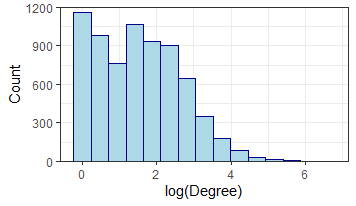
\includegraphics{Images/degree_dist.png}
\caption{Distribution of log degree in the Twitch dataset.}
\label{fig:degree}
\end{figure}

\subsection{Simulated treatment details} \label{apx:covbal}

Figure~\ref{fig:neighbourhood} shows the distribution of proportion and log sum neighbourhood treatments in one simulated dataset. For proportion $G_i$, the mean and median are 0.59 and 0.63, respectively. The standard deviation is 0.30, and the first and third quartiles are 0.44 and 0.80, respectively. For sum $G_i$, the values range from 0 to 489 with a median of 3, a mean of 6.3, and a standard deviation of 14.7. The first and third quartiles are 1 and 7, respectively.

\begin{figure}[H]
\centering
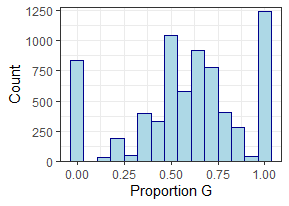
\includegraphics{Images/prop_g_dist.png}
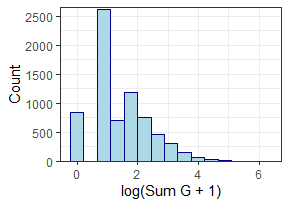
\includegraphics[trim={0.6cm 0 0 0},clip]{Images/sum_g_dist.png}
\caption{Distribution of proportion and log sum neighbourhood treatments in one simulated dataset. Note that for the sum plot, 1 was added to every $G_i$ before taking the log due to the presence of zeros.}
\label{fig:neighbourhood}
\end{figure}

Tables~\ref{tab:indcovbal} and \ref{tab:nbrcovbal} show the covariate balance across treatment arms in one simulated dataset. The standardized difference \parencite{Austin:2011} is computed as
\[
\text{Stand. Diff.} = \frac{\bar{X}_{Z=1} - \bar{X}_{Z=0}}{\sqrt{\frac{s^2_{Z=1}+s^2_{Z=0}}{2}}}
\]
for continuous variables (all but game1, game2, and $Z_i$) where $s^2$ is the variance for the corresponding group, and otherwise computed as
\[
\text{Stand. Diff.} = \frac{\bar{X}_{Z=1} - \bar{X}_{Z=0}}{\sqrt{\frac{\bar{X}_{Z=1}(1-\bar{X}_{Z=1})+\bar{X}_{Z=0}(1-\bar{X}_{Z=0})}{2}}}
\]
for binary variables. Some works in the literature interpret a standardized difference of less than 0.1 (10\%) as the covariate being balanced across treatment arms \parencite{Normand:2001}.

\begin{table}[H]
\centering
\begin{tabular}{@{}lrrr@{}}
\toprule
Variable & $\bar{X}_{Z=1}$ & $\bar{X}_{Z=0}$ & Stand. Diff. \\
\midrule
game1 & 0.683 & 0.326 & 0.763 \\
game2 & 0.763 & 0.176 & 1.454 \\
Ngame1 & 0.486 & 0.466 & 0.061 \\
Ngame2 & 0.620 & 0.586 & 0.114 \\
Degree & 10.757 & 8.717 & 0.088 \\
Proportion $G_i$ & 0.604 & 0.569 & 0.118 \\
Sum $G_i$ & 6.979 & 5.365 & 0.106 \\
\bottomrule
\end{tabular}
\caption{Covariate balance across individual treatment arms.}
\label{tab:indcovbal}
\end{table}

\begin{table}[H]
\centering
\begin{tabular}{@{}l@{\hskip 3em}rrr@{\hskip 3em}rrr@{}}
\toprule
Variable & $\bar{X}_{G\geq0.5}$ & $\bar{X}_{G<0.5}$ & Stand. Diff. & $\bar{X}_{G\geq3}$ & $\bar{X}_{G<3}$ & Stand. Diff. \\
\midrule
game1 & 0.558 & 0.471 & 0.175 & 0.723 & 0.334 & 0.846 \\
game2 & 0.542 & 0.461 & 0.162 & 0.555 & 0.483 & 0.144 \\
Ngame1 & 0.553 & 0.267 & 0.938 & 0.564 & 0.385 & 0.559 \\
Ngame2 & 0.669 & 0.430 & 0.818 & 0.631 & 0.580 & 0.174 \\
Degree & 11.694 & 4.897 & 0.371 & 16.905 & 2.432 & 0.701 \\
$Z_i$ & 0.608 & 0.526 & 0.167 & 0.677 & 0.490 & 0.385 \\
\bottomrule
\end{tabular}
\caption{Covariate balance across dichotomized neighbourhood treatment arms. For sum $G_i$, the median 3 was taken as the threshold.}
\label{tab:nbrcovbal}
\end{table}

\subsection{Number of subclasses investigation} \label{apx:subclass}

We conducted a small investigation into the effect of the number of subclasses on the RMSE of the individual and all covariate-adjusted estimators and of the GPS estimator \parencite{Forastiere:2021}. Figure~\ref{fig:subclass} shows the effect of the number of subclasses on the mean RMSE over 25 datasets simulated with high interference and either proportion neighbourhood treatments (left) and sum neighbourhood treatments (right). The same 25 datasets were used across numbers of subclasses in each plot. Our results suggest that while the five subclass recommendation by \textcite{Rosenbaum:1984} does not necessarily lead to the smallest RMSE, the RMSE of most estimators do not change significantly with more than five subclasses (the one exception being the estimator that adjusts for all covariates in the sum neighbourhood treatment case). It is also interesting that increasing the number of subclasses does not necessarily reduce the RMSE, notably with the all-covariates and the GPS estimators where the RMSE spikes at four subclasses.

\begin{figure}[ht]
\centering
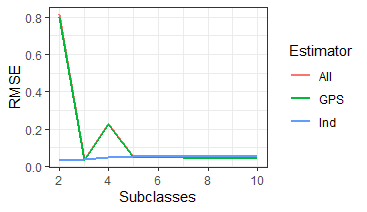
\includegraphics[trim={0.2cm 0 2.5cm 0},clip]{Images/subclasses_prop.png}
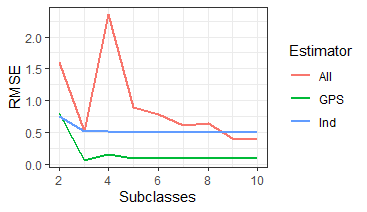
\includegraphics[trim={0.55cm 0 0.2cm 0},clip]{Images/subclasses_sum.png}
\caption{RMSE as the number of subclasses changed for three treatment effect estimators. The left plot shows the mean RMSE over 25 datasets simulated with proportion neighbourhood treatment and the right for those with sum neighbourhood treatments. The RMSE of the all-covariates and the GPS estimators follow similar trajectories in the left plot.}
\label{fig:subclass}
\end{figure}


\end{document}